\documentclass{article}

\usepackage{graphicx}
\usepackage{amsmath}
%% Key definitions for text elements. USE THEM
\def\secref#1{Sec.~\ref{#1}}
\def\figref#1{Fig.~\ref{#1}}
\def\tabref#1{Tab.~\ref{#1}}
\def\eqref#1{Eq.~(\ref{#1})}
\def\algref#1{Alg.~\ref{#1}}
\def\appref#1{App.~\ref{#1}}

\newcommand\etal{\emph{et al.}}

\title{\LARGE \bf Semantic Mapping Pipeline}

\begin{document}
	
	\maketitle	
	
	\begin{figure}[htbp]
		\centering
		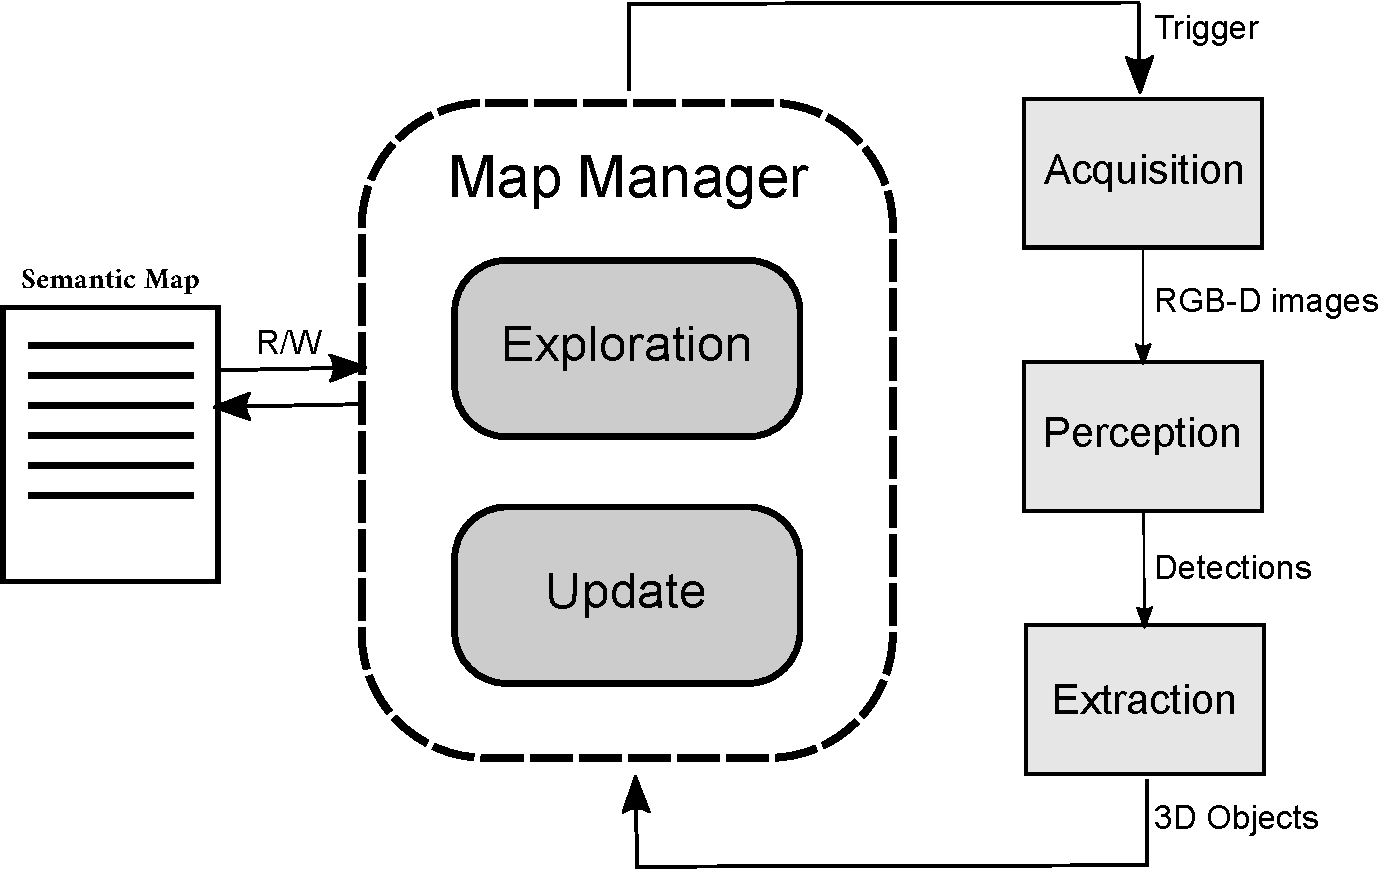
\includegraphics[width=\linewidth]{pics/drawing-crop.pdf}
		\caption{System pipeline.}
		\label{fig:pipeline}
	\end{figure}
	
	\section*{Semantic Map}
	
	In our system, a semantic map $\mathcal{SM} = \{\mathbf{O}_i\}_{i=1 \dots N}$ is a collection of 3D objects, where each object $\mathbf{O}_i$ is a tuple defined by:
	
	\begin{equation}
			 <\text{Type},\text{Pose3D},\text{Size3D},\text{Model}>.
	\end{equation}
	
	\noindent
	Possible operations on the map are:
	
	\begin{itemize}
		\item query for object: given an object it's possible to check if it's already present in the map
		\item update object: allows to update an object present in the map with a new observation
		\item add object: allows to add an object to the map if it's seen for the first time
		\item render map: builds a 3d model from the collection of objects, this function can be used for navigation and visualization.
		\item serialize/deserialize: these functions allow to save a map on disk and to load it for later use.
	\end{itemize}
	
	\section*{Map Manager}
	
	The map manager has the task of incrementally updating the semantic map with new observations coming from sensors.
	
	\subsection*{Update}
	
	The update of the map can be done by registering a local frame with the global model. To this end, it's necessary to know the pose of the robot relative to the global reference frame. This information may be provided by SLAM systems, while, in simulation environments is known. Once objects are transformed in global frame, data association is performed to find correspondences between local and global map (object tracking) and update the global map accordingly.
	
	\begin{description}
		\item{\bf Data association:} finds which objects in the global map correspond to the one observed in the local map. This correspondence is evaluated through a similarity measure. So that, finding a corresponding object can be casted into a nearest-neighbor search. Usually, similarity is computed through euclidean distance. In our problem, it's possible to leverage also semantic information. In case of a limited number of objects, brute-force is a reasonable technique to choose. In the simulated environment, the knowledge of the semantic class is perfect. In real world scenarios, object detectors return a probability distribution over semantic labels. In the first case, the corresponding object is the closest one with the same type. In the second case, euclidean distance could be weighted with class probabilities to represent a form of similarity measure.
		
		\item{\bf Update:} integrates incoming information from local map into global map. Input: maps, correspondences. Output: updated global map. Steps: for each object in local map check if it's already been seen, yes: merge, no: add to map. This strategy may fail in case of false positives returned by data association. Possible solution:  aging scheme.
	\end{description}
	
	\subsection*{Exploration}
	
	The exploration module has the task of navigating the robot in a way to improve its current knowledge of the environment. To do so, it receives the current belief of the problem state, i.e. map and robot pose, and computes a goal pose that maximizes a cost function based on different criteria, e.g., navigation cost, information gain, and so on.
	
	\section*{Processing}
	
	Our processing pipeline is made of three modules that exchange data structures among each other to build and maintain the semantic map.
	
	\subsection*{Acquisition}
	
	This module is in charge of triggering the acquisition of sensor data to update the semantic map. Different acquisition strategies may be impemented:
	
	\begin{itemize}
		\item Time based
		\item Space based
		\item Information based
		\item Human-in-the-loop
	\end{itemize}
	
	\subsection*{Perception}
	
	The perception module is in charge of localizing and classifying objects in the current frame to label each image pixel with its semantic class. More formally, given an image $I \subset \mathbf{N}^{3 \times 2}$ and a set of semantic labels $\mathcal{L} = \{l_i\}_{i=1 \dots L}$, computes an assignment of labels $l_i \in \mathcal{L}$ to each image pixel $x = (u,v) \in I$ .
	
	\subsection*{Extraction}
	
	Feature extraction is performed by taking the output of the perception module and building a 3D object (atomic entity of the map) from each detection. After that, by knowing the pose of the robot in the global frame, it's possible to transform the extracted objects in the global frame to find correspondences (data association).
	
	

	
\end{document}